% -------------------------------------------------------------------------------------------------
%      MDSG Latex Framework
%      ============================================================================================
%      File:                  introduction-[UTF8,ISO8859-1].tex
%      Author(s):             Michael Duerr
%      Version:               1
%      Creation Date:         30. Mai 2010
%      Creation Date:         30. Mai 2010
%
%      Notes:                 - Example chapter
% -------------------------------------------------------------------------------------------------
%
\chapter{Approach}\label{sec:Concept}
- What is your plan? \\
- How do you proof that it worked? -> Metric and Experiments


\section{Coloring Environment}\label{env}
\marginpar{origin and intro}
% Introduce Gridworld, Agent actions, goal etc.
A RL environment is a versatile and unbiased instance, that can can be used to visualize agent behavior and environmental changes.
% Although a human visualization is optional, agents need to have some sort of understanding what state they are acting in. 
In figure \ref{fig:env}, the environment used in this work is presented. It originated from an openAI project called ``Minimalistic Gridworld Environment'' \cite{chwi18}, which is designed for one agent whose main goal is to solve labyrinth puzzles. For the purpose of this research however, the environment is changed heavily, becoming the ``Coloring Environment''. Multiple agents can act in the new instance to try and achieve a new goal - to color all walkable cells.

\begin{figure}[hpbt]
    \centering
    %%----start of first subfigure----
    \subfloat[Human visualization of the coloring environment. A dot represents one agent. Cells change their color when agents moves  on them.]{
        \label{fig:env} %% label for first subfigure
        \includegraphics[width=0.35\linewidth]{pictures/Gridworld}}
    \hspace{0.01\textwidth}
    %%----start of second subfigure----
    \subfloat[Simplified agent observation of the current environment state. The number 1 represents a colored cell.]{
        \label{fig:bin_env} %% label for second subfigure
        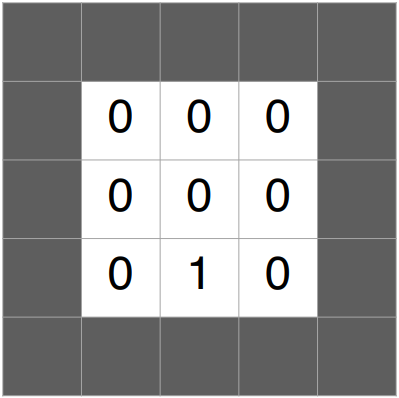
\includegraphics[width=0.35\linewidth]{pictures/binary_gridworld}}
    \caption[Coloring Environment]{Representations of the coloring environment}
    \label{fig:multipic_env} %% label for entire figure
\end{figure}

\marginpar{cell objects}
Figure \ref{fig:bin_env} shows a simplified environment observation an agent processes each timestep. Every environment cell holds information about the object it represents, being either Walls, Floors or Agents. Furthermore, each object class contains information about its current color, whether or not it is accessible for an agent and, in case of a floor tile, if it is colored.


\subsection{Compositions}
\marginpar{compositions}
When multiple agents are placed in the coloring environment together, there are several ways how they will behave towards each other. Depending on the setting, even the environment distinguishes how certain actions affect the state. Per default agents will try to work together, to reach the environment goal. Alternatively, they could work independently or even compete with each other.

\marginpar{floor coloration}
Floor cells keep the coloration state in binary form, as displayed in \ref{fig:bin_env}, with a 1 signalizing that the cell is colored. The environment reacts to agent movements by coloring the cells they visit. Agents successfully solve the environment once all fields are colored. Otherwise agents loose by using up a limited amount of steps.

\marginpar{bit switching}
If a cell is already in coloration state 1 and an agent walks over it again the bit is switched and the cell is reset to 0, removing its coloration. Besides moving up, down, left and right an agent can also execute the action wait, to stay in place.

\marginpar{cooperative multiagents}
Each agent has a different random color. In the human representation (figure \ref{fig:env}) cells adopt the color of the agent that walks over it. The primary focus in cooperative agent compositions is only the binary state. All agents receive the same maximum reward when the grid is fully colored, making it irrelevant what colors the cells have.

\marginpar{mixed-motive multiagents}
The opposite is the case in competitive scenarios. In mixed-motive settings for example, agents only gain high rewards once the grid is fully colored, with the twists that it depends on their contribution. The final reward is generated by looking up the percentage a color is present and assigns that value as reward to the corresponding agent.

\marginpar{competitive multiagents}
In a fully competitive scenario the reward calculations stay the same, only disabling the bit switching. Therefore, agents can directly capture already colored cells when they walk over them. Hence, taking over the cells of the opponents is beneficial, since it increases the color presence of the own color, leading to a higher final reward.

\marginpar{comparison multiagents}
In comparison, the mixed-motive scenario shows no advantages resetting colored cells of others. In this case the cell is not captured and the agent is also punished with a small penalty when doing that. Hence, the mixed-motive setting represents the independent agent composition.

\subsection{Observation}
\marginpar{what the agent sees}
The observations agents receive from the environment are always generated from their individual point of view and only contain a restricted area around them. In large environments this feature increases the difficulty but at the same time reflects the reality. An example for a proper observation of an agent is shown in \ref{fig:agent_obs}. This observation represents the internal state of the human representation of image \ref{fig:env}.

\begin{figure}[hpbt]
    \centering
    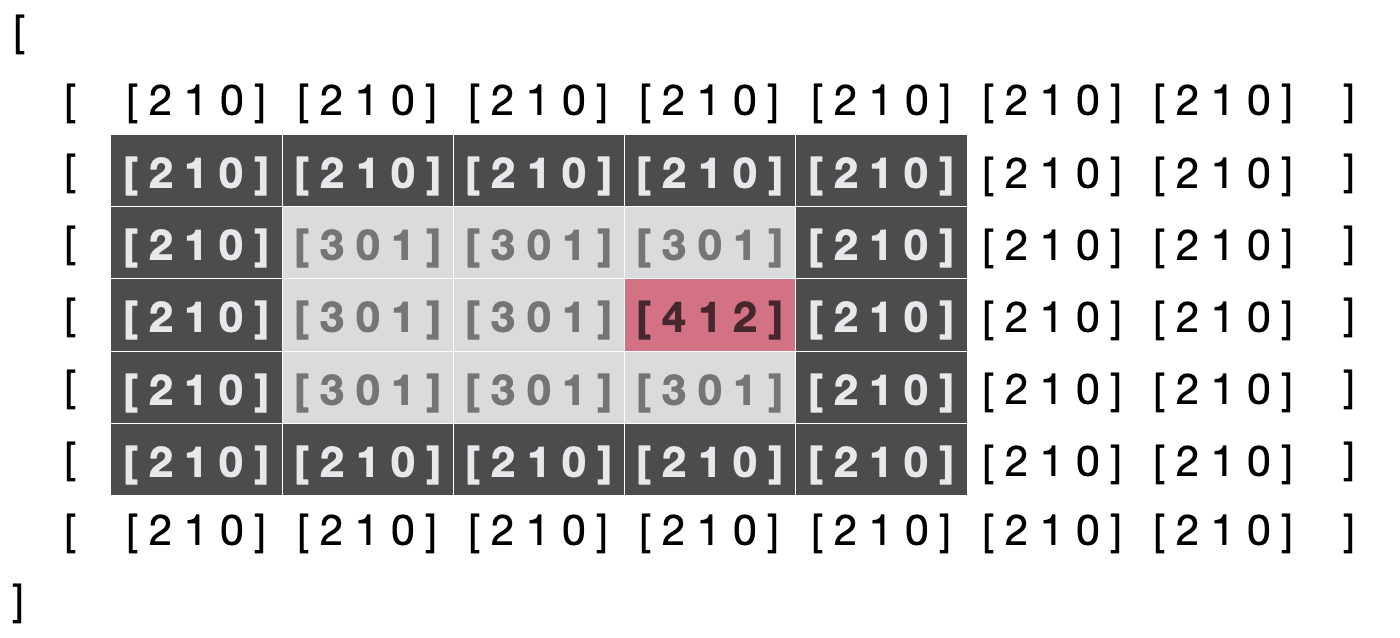
\includegraphics[width=0.8\textwidth]{pictures/agent_observation}\\
    \caption[agent observation]{The internal agent observation}\label{fig:agent_obs}
\end{figure}

\marginpar{description}
Per default the agent has a view size of a seven by seven grid, represented in a three dimensional array, similar to a picture with rgb information. Here, all bold entries are part of the grid and the colored array is the agent position. All remaining grayed out elements are additions to the observation in order to standardize the observation size.

\marginpar{dimensions}
The first dimension of the array contains the whole observation, the second dimension represents each grid column of \ref{fig:env}, starting from the top left and the third dimension encodes each cell. The encoding first defines the object type with 1 being just an empty cell, 2 shows a wall, 3 a floor tile and 4 an agent. Second, the coloration status is visible. Since agents can not walk onto walls, that object type has a coloration state of 1 per default.
% This also reduces the complexity of checking for a fully colored grid by just looking at all coloration states, regardless of the object type.

\marginpar{cell encoding colors}
The third encoding signalizes the color of a cell. To better distinguish the types in the human representation, walls are 0 for the color black and floors are initially white with encoding 1. Each agent is assigned a number from 2 upwards which in turn stands for a randomly generated color. The Floor color encoding is overwritten with the agents color when the cell is captured.

\section{Reward Calculations}
\marginpar{activation line}
The allocation of rewards is closely related to the composition of the agents, which can be specified by the user in training or visualization runs. In addition the environment shape can be set, a number of agents placed and more. A basic example command for a training run is shown in listing \ref{lst:command}.

\begin{lstlisting}[float=htp,caption=Exemplary command to execute training with three agents in a coloring environment with PPO as algorithm,label=lst:command,language=bash, numbers=left, numberstyle=\tiny, numbersep=8pt, escapeinside={//@}{@//},xleftmargin=3ex,xrightmargin=1ex]
$ python -m Coloring.scripts.train
    --algo ppo
    --model ppo-training
    --env Empty-Grid-v0 
    --grid-size 9 
    --agents 3 
    --max-steps 350
    --setting mixed-motive
\end{lstlisting}

\marginpar{command algo and model}
The ``algo'' parameter can be either ``ppo'' or ``dqn'' to choose a learning algorithm. This argument is the only required setting for training. All other configurations, including those not listed in \ref{lst:command}, have default values and are discussed in the sections \ref{learning_process} and \ref{market_settings}. An overview of all training parameters and their default values is listed in Appendix \ref{ax:training_params}. The model defines the name for a destination folder, in which all logs, recordings and status updates are stored.

\marginpar{command env}
Line 4 and 5 configures the environment. Alternatively to the empty grid option of ``env'', as shown in figure \ref{fig:env}, four homogeneous rooms can be generated with ``FourRooms-Grid-v0'' to increase the difficulty. The rooms are of the same size and each room is accessible to all adjoining neighbors by one opening, which is random and changes in each episode. The overall size of the grid is set in Line 5, however all grids in every layout option have outer walls that narrow the area in which agents can move.

\marginpar{settings}
The amount of agents that act in the environment is set through the argument ``agents'' and the maximum quantity of steps they can execute is defined with ``max-steps''. To gain the maximum reward, the agents need to color the whole field before they run out of steps. Lastly, the argument ``setting'' specifies the composition of the agents. If no setting is set the agents work cooperatively. In the example of \ref{lst:command} the setting ``mixed-motive'' is chosen. The last option here is ``mixed-motive-competitive''. % and ``percentage''.

\marginpar{environment reward}
In each step agents get separate environment rewards based on their coloration. Agents that color a field receive a reward of 0.1, whereas agents that reset a field get a penalty of -0.1. In the competitive mode agents can not reset fields and therefore receive no penalty. In this case the contrary happens, capturing cells of other agents, yield a positive reward of 0.1. Agents that just wait get a reward of 0. All rewards are written into a list and returned by the environment. The position in the list indicates the receiving agent. In algorithm \ref{algo:step_reward} the process of adapting the initial environment rewards with the specified training arguments is summarized.

\begin{algorithm}[H]
    \DontPrintSemicolon
    observations, rewards, done, info = environment.step(actions)\;
    \If{cooperative setting}{
        rewards = calculate one cooperative reward
    }
    \If{market specified}{
        rewards = execute market actions and return transaction rewards\;
    }
    \If{done}{
        rewards = calculate final rewards
    }
    \textbf{return} observations, rewards, done, info\;
    \caption{Reward calculation each step}\label{algo:step_reward}
\end{algorithm}

\marginpar{coop reward}
First, for a cooperative setting a new homogeneous reward needs to be calculated out of the environment rewards. The calculation for that is summing up all list values and checking if they exceed an upper or lower bound. If that is the case then the new reward is set to the corresponding limit, otherwise the sum is taken as is. This step is necessary, due to more participating agents possibly leading to a really big or really small sum. This in turn could decrease the importance of the final reward for reaching the environment goal. For settings that contain ``mixed-motive'' this calculation is skipped, since here each agent is responsible for its own environment reward.

\marginpar{market actions}
Second, the market transactions are executed, if a shareholder or action market is specified. The market details are discussed in Section \ref{market_settings}. One thing to note here is that agents can execute transactions in each step, spending their current reward on items for sale or receive the purchase price from buyers. Therefore the rewards change in this step too.

\marginpar{done calculations}
Lastly, the final reward is calculated when done is set to true. That is the case when the environment goal is reached or all steps are used up. Algorithm \ref{algo:final_reward} shows the executed calculations of that case. Again the first thing to check is whether the agents work together. If not, each agents' grid coloration percentage, based on their color presence, is added to the individual reward. Otherwise the environment goal condition is checked for the cooperation mode. If the grid is fully colored the value one is added to each agent reward, since everyone gets the same feedback. Finally, the last market calculations are included into the rewards, see chapter \ref{market_settings} for details.

\begin{algorithm}[H]
    \DontPrintSemicolon
    \eIf{mixed setting}{
        \For(){each agent}{
            rewards[agent] += agent color percentage on the field
        }
    }{// cooperative setting \;
        \If{grid fully colored}{
            \For(){each agent}{
                // add the maximum value of 1 to each agent reward \;
                rewards[agent] += 1
            }
        }
    }
    \If{market specified}{
        rewards = final market adjustments executed on rewards
    }
    \textbf{return} rewards\;
    \caption{Final reward calculation}\label{algo:final_reward}
\end{algorithm}


\section{Learning Process}\label{learning_process}
% \subsection{Base Class}
\marginpar{Independent learning}
In order to compare different settings and agent compositions easily, each agent manages its own learning improvement, observation and action selection. Therefore all calculations and estimations are executed independently, for instance policy updates and value estimations. They also set up their own neural networks and optimizers and update them only with their own values. However, observations still connect the agent experiences, by including the positions of all agents on the grid and reacting to their joint actions in each step.

\marginpar{process structure}
Depending on the learning algorithm the corresponding class is instantiated by the training script, as shown in Figure \ref{fig:training}. PPO and DQN both extend a base class that provides some abstract methods and a multiprocessing operation to execute actions on several environments at once. If specified, the base class returns data, allowing the training script to create recordings and log files to enable evaluation.

\begin{figure}[hpbt]
    \centering
    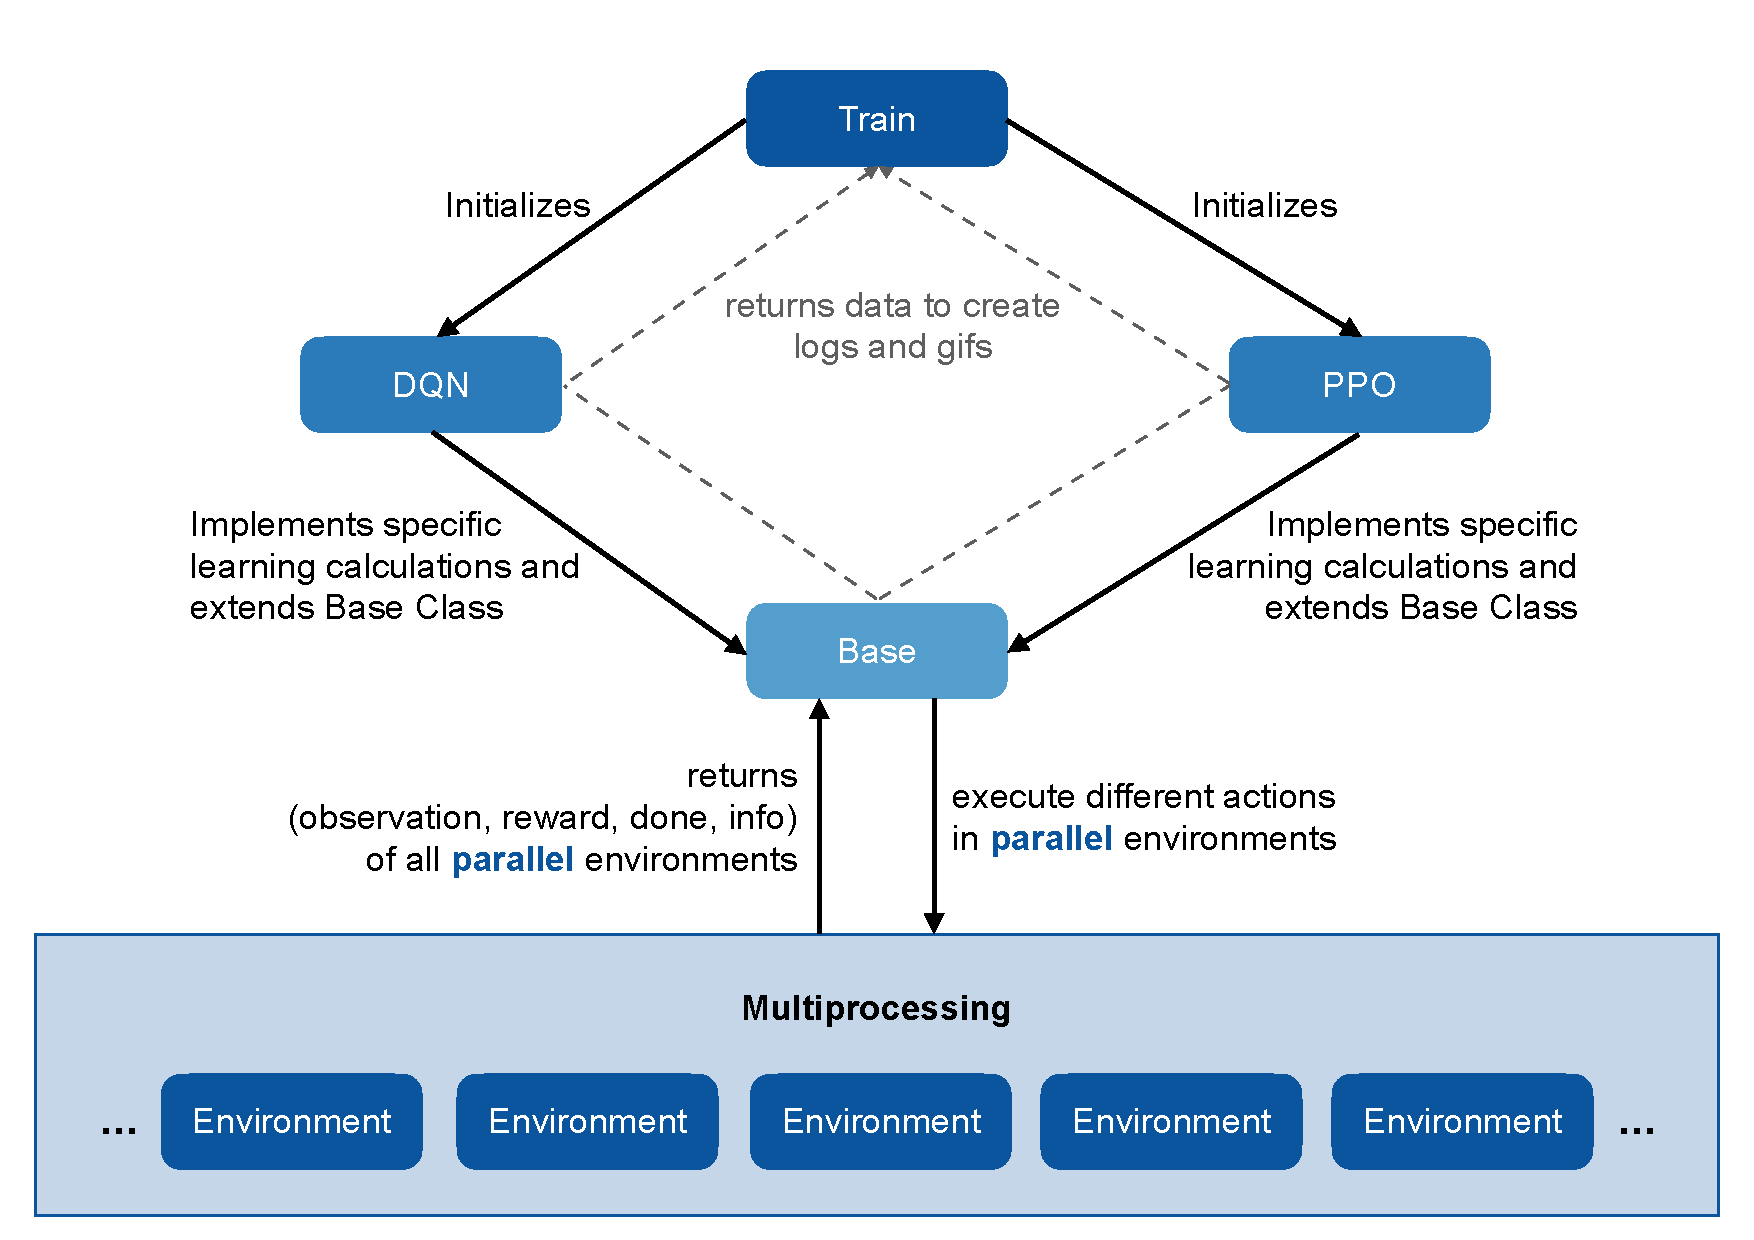
\includegraphics[width=0.9\textwidth]{pictures/training}\\
    \caption[The training structure]{The training structure}\label{fig:training}
\end{figure}

\marginpar{training setup}
First, the training begins by creating n environments based on the \verb|--procs| setting of the training command, see Appendix \ref{ax:training_params} for the parameter list. Each environment has the same configurations, set through the arguments, for example \verb|--grid-size|, \verb|--agents| and \verb|--agent-view-size|. Second, the amount of \verb|--frames| is taken from the parameters, defining a loop until that number is reached. In this case frames are equivalent to agent steps. During the loop, the defined training algorithm \verb|--algo| is executed.

\marginpar{base class}
Since both, DQN and PPO have similar procedures, they share the base class. In it experiences are gathered through a certain amount of actions which are executed on parallel environments. The action amount is set with \verb|--frames-per-procs|. During that period details like gained rewards, environment observations, actions and more are stored in base class variables that are accessible by the learning algorithms. When all experience actions are executed, the base variables are reset and log values are returned, as shown in Figure \ref{fig:training}. Afterwards the frame counter in the training script is updated with the amount of \verb|--frames-per-procs|. The training loop ends when the frames counter is greater than \verb|--frames|. Otherwise more experience batches are gathered.

\marginpar{action selection}
Both learning algorithms implement their own action selection method. The PPO implementation relies on an actor-critic neural network, letting the actor part calculate a probability distribution of the action space. In case of DQN a linear neural network assigns Q values to actions, choosing the maximum value with an epsilon greedy practice. In both variants the action selection results in one action for each agent and for each environment. The environments finally receives a joint action array that merged the agents action.

\subsection{DQN}
\marginpar{replay memory}
Unlike PPO, DQN saves a quadruple of information each frame into a replay memory. The four parts of said quadruple consist of the the executed actions of that timestep, the returned rewards and both the previous and new observation of the parallel environments. Until the frame amount of \verb|--initial-target-update| is reached, DQN only gathers such memory entries.

\marginpar{target update}
After exceeding the \verb|--initial-target-update|, DQN starts to learn. Each frame a batch of size \verb|--batch-size| is selected by randomly picking entries from the replay memory. Then this batch is used to apply Q-learning updates to the experience samples, enhancing the training network. Every \verb|--target-update| amount of frames this training network is copied into the target network to enhance the action selection while keeping the algorithm stable.

The action selection itself is also enhanced during the training, by decreasing the $\epsilon$ gradually through $\epsilon = \epsilon_{end}+(\epsilon_{start}-\epsilon_{end})*e^{-\frac{frames}{decay}}$. This ensures exploration in the early phase. A high $\epsilon$ leads to actions that are picked at random. In the later course as the amount of frames increase, the $\epsilon$ is gets smaller. In this case, the chance to select actions based on their Q values rises, which exploits the gathered experiences. Through \verb|--epsilon-start| and \verb|--epsilon-end| min and max values are set, and \verb|--epsilon-decay| defines the speed of reduction.

\subsection{PPO}
5. berechnung ppo + parameter
6. berechnung dqn + parameter
Independent learning! each agent has own actor/critic or complete network
agent observation explanation
PARAMETERS!
16 parallel envs with frames,
nn takes observation
how the values and percentages are calculated

\section{Market Settings}\label{market_settings} % Agent Compositions
TODO: RL Skizze \ref{fig:rl_cycle} erweitern wie agenten pro schritt am markt handeln und was in done passiert!
\marginpar{MARL Challenges}
Each of the three compositions presented in chapter \ref{env} lead to learning problems or game losses. Cooperation may reward misbehavior, namely field resetting, leading to the CAP of chapter \ref{CAP}. In mixed-motive or fully competitive settings the overall goal may be never reached due to greediness or disorder. This research further compares the effects of markets not only on competitive settings as suggested by Schmid et al. \cite{scbe21}, but rather on all three configurations.

\marginpar{action space}
As mentioned earlier, agents have five possible action choices each timestep: moving up, down, left, right or simply to wait. Adding a market to the stochastic game expands this one dimensional action space into a three dimensional action space.
- am

- am-goal

- am-goal-no-reset

- sm

- sm-goal

- sm-goal-no-reset

